\documentclass[tikz,border=8pt]{standalone}
% Shared styles for the Hands-On 4 diagrams. Colours match the Hands-On 1 diagrams.
\usepackage{amsmath,amssymb}
\usetikzlibrary{positioning,calc,arrows.meta,decorations.pathreplacing,shapes.geometric}
\definecolor{tensorblue}{HTML}{3274B5}
\definecolor{envblue}{HTML}{1E4C7C}
\definecolor{opteal}{HTML}{357A76}
\tikzset{
  leg/.style={line width=1.7pt},
  thinedge/.style={line width=1.0pt},
  tensor/.style={circle,draw,line width=1.5pt,fill=tensorblue,minimum size=9mm,inner sep=0},
  vertex/.style={circle,draw,line width=1.0pt,fill=white,minimum size=6mm,inner sep=0,font=\small},
  copy/.style={circle,draw,line width=1.5pt,fill=black,minimum size=3.6mm,inner sep=0},
  op/.style={rectangle,draw,line width=1.5pt,fill=opteal,minimum size=5.6mm,inner sep=0},
  % messages are triangles pointing in the direction the message travels
  msg/.style={isosceles triangle,isosceles triangle apex angle=75,draw,line width=1.5pt,fill=envblue,inner sep=0,
              minimum width=8mm,minimum height=10mm,shape border rotate=0},
  msgl/.style={msg,shape border rotate=180},
  msgu/.style={msg,shape border rotate=90},
  msgd/.style={msg,shape border rotate=270},
  % a matrix message: a slightly larger triangle, its two legs fan out from it
  msgmat/.style={msg,minimum width=10mm,minimum height=13mm},
  lab/.style={font=\large},
  code/.style={font=\ttfamily\large},
  arrow/.style={-{Latex[length=3mm]},line width=1.2pt},
}

\begin{document}
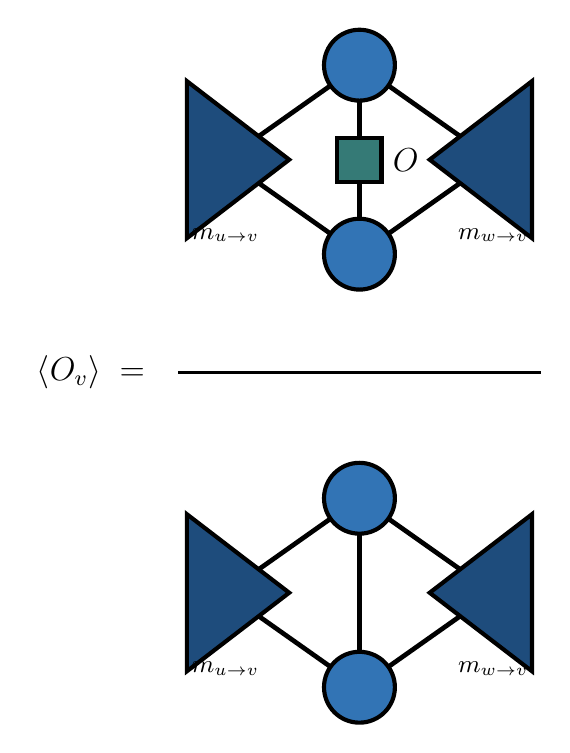
\begin{tikzpicture}
  % one site of the chain with its two incoming matrix messages; the operator sits on the
  % physical leg between the ket and the bra
  \newcommand{\site}[2]{% #1 = y offset of the ket row, #2 = draw the operator (1) or not (0)
    \begin{scope}[yshift=#1]
      \coordinate (L) at (0,1.2); \coordinate (R) at (3.4,1.2);
      \coordinate (k) at (1.7,0); \coordinate (b) at (1.7,2.4);
      \draw[leg] (L) -- (k); \draw[leg] (L) -- (b);
      \draw[leg] (R) -- (k); \draw[leg] (R) -- (b);
      \draw[leg] (k) -- (b);
      \node[msgmat] at (L) {};
      \node[msgmat,shape border rotate=180] at (R) {};
      \node[tensor] at (k) {}; \node[tensor] at (b) {};
      \ifnum#2=1 \node[op] at (1.7,1.2) {}; \node[lab,anchor=west] at (2.0,1.2) {$O$}; \fi
      \node[lab,anchor=north] at (0,0.45) {\small$m_{u \to v}$};
      \node[lab,anchor=north] at (3.4,0.45) {\small$m_{w \to v}$};
    \end{scope}
  }
  \node[lab,anchor=east] at (-0.9,0.4) {$\langle O_v \rangle \;=$};
  \site{1.9cm}{1}
  \draw[line width=1.1pt] (-0.6,0.4) -- (4.0,0.4);
  \site{-3.6cm}{0}
\end{tikzpicture}
\end{document}
